% easier quotes
\newcommand{\gqq}[1]{\glqq#1\grqq}

\section{Präventive Verteidigungsmaßnahmen}

\begin{frame}{Präventive Verteidigungsmaßnahmen}
        \begin{block}{Mehrschichtige Sicherheitsstrukturen}
                \begin{itemize}[<+->]
                        \item Experten: Sicherheitslücken \textbf{nicht} zu 100\% ausschließbar
                        \item Können aber durch mehrschichtige Sicherheitsstrukturen migriert werden
                        \item Torvalds: \gqq{The only real solution to security is to admit that bugs happen, and then mitigate them by having multiple layers, so if you have a hole in one component, the next layer will catch the issue.} \footnotemark 
                \end{itemize}
        \end{block}
        
        \setbeamerfont{footnote}{size=\tiny}
        \footnotetext{Quelle: http://www.eweek.com/enterprise-apps/linus-torvalds-talks-linux-security-at-linuxcon.html\\(Besucht am 13.12.2015)l}
        \setbeamerfont{footnote}{size=\footnotesize}
\end{frame}

\begin{frame}{Präventive Verteidigungsmaßnahmen}
        \begin{block}{Zugriffskontrolle}
                \begin{itemize}[<+->]
                        \item Zugriffskontrolle kann eine Schicht sein
                        \item Zentrale Frage: Wer darf welche Daten lesen, schreiben, ausführen?
                        \item Drei grundlegene Modelle:
                        \begin{itemize}[<+->]
                                \item Mandatory Access Control (MAC)
                                \item Discretionary Access Control (DAC)
                                \item Role-based Access Control (RBAC)
                        \end{itemize}
                \end{itemize}
        \end{block}
\end{frame}

\begin{frame}{Präventive Verteidigungsmaßnahmen}
        \begin{block}{AppArmor}
                \begin{itemize}[<+->]
                        \item Einfache Umsetzung von Mandatory Access Control (MAC)
                        \item Schränkt die Rechte von Applikationen ein
                        \item Im Vergleich zu SELinux einfache Konfiguration
                        \item Schutzziele: Vertraulichkeit, Integrität und Verfügbarkeit
                \end{itemize}
        \end{block}
\end{frame}

\begin{frame}{Präventive Verteidigungsmaßnahmen}
        \begin{block}{Sandboxing}
                \begin{itemize}[<+->]
                        \item Ziel: Abgrenzung von Software und Hardware
                        \item Komplexität reduzieren (in einer Sandbox läuft gewöhnlich genau eine Anwendung)
                        \item Schnell \& einfach wiederherstellbar (Disaster Recovery)
                        \item Einsatz: BIND unter UNIX, Google's Browser Chrome, ...
                        \item Verschiedene Möglichkeiten der Virtualisierung
                \end{itemize}
        \end{block}
\end{frame}

\begin{frame}{Präventive Verteidigungsmaßnahmen}
        \begin{figure}
                \centering
                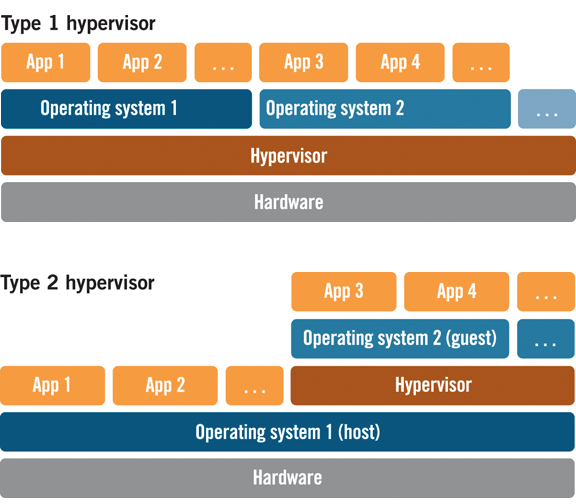
\includegraphics[width=0.55\textwidth]{assets/hypervisor}
                \caption{Hypervisor Typen \footnotemark}
        \end{figure}

        \setbeamerfont{footnote}{size=\tiny}
        \footnotetext{Quelle: http://www.virtzone.net/the-difference-between-a-type-2-hypervisor-and-a-type-1-hypervisor/\\(Besucht am 13.12.2015)l}
        \setbeamerfont{footnote}{size=\footnotesize}
\end{frame}

\begin{frame}{Präventive Verteidigungsmaßnahmen}
        \begin{block}{Docker}
                \begin{itemize}[<+->]
                        \item Was sind Container?
                        \begin{itemize}[<+->]
                                \item \textbf{\gqq{$\sim$chroot on steroids}}
                                \item Ein Set von Prozessen
                                \item Isoliert\footnotemark vom Rest der Maschine
                                \item Per \textit{namespaces} eigene private Resourcen
                                \item Per \textit{cgroups} Limitierung von Resourcen möglich
                        \end{itemize}
                        \item Container: Gibt es seit Jahrzehnten
                        \item LXC (Linux Container): Gibt es seit Jahren
                        \item $\rightarrow$ Docker vereinfacht die Verwendung von LXC 
                \end{itemize}
        \end{block}

        \setbeamerfont{footnote}{size=\tiny}
        \footnotetext{Teilen sich den Kernel}
        \setbeamerfont{footnote}{size=\footnotesize}
\end{frame}

\begin{frame}{Präventive Verteidigungsmaßnahmen}
        \begin{block}{Wie sicher ist Docker?}
                \begin{itemize}[<+->]
                        \item \gqq{LXC is not yet secure. If I want real security I will use KVM.} Ben Berrangé (LXC Maintainer) 2011\footnotemark
                        \item Seit dem hat sich aber einiges getan
                        \item Kernel namespaces sind über 5 Jahre alt und damit relativ ausgereift
                        \item Docker startet Container mit sehr begrenzten \textit{Capabilities}
                        \item Prozesse im Container sollten dennoch nicht als \textit{root} laufen
                \end{itemize}
        \end{block}

        \setbeamerfont{footnote}{size=\tiny}
        \footnotetext{Quelle: https://blog.docker.com/2013/08/containers-docker-how-secure-are-they/\\(Besucht am 13.12.2015)l}
        \setbeamerfont{footnote}{size=\footnotesize}
\end{frame}

\begin{frame}{Präventive Verteidigungsmaßnahmen}
        \begin{block}{Fazit}
                \begin{itemize}[<+->]
                        \item Zwar sind Docker Container inzwischen relativ sicher
                        \item Dennoch sollten zusätzliche Sicherheitsschichten verwendet werden
                        \item $\rightarrow$ Kombination mit z.B. AppArmor
                        \item Auch wenn zusätzliche Sicherheitsschichten einen \textit{Overhead} verursachen,
                        \item so lohnt sie sich am Ende doch oft 
                \end{itemize}
        \end{block}
\end{frame}

